







\section{Introduction aux directions de descente}
Commençons par d\'efinir le contexte avec un peu de vocabulaire et les hypoth\`eses faites sur le probl\`eme. Puis nous allons analyser
 les concepts n\'ecessaires pour la suite. 
\subsection{Hypoth\`eses de travail}
Dans l'ensemble du texte, nous faisons deux hypoth\`eses : la continuit\'e et la diff\'erentiabilit\'e.
Soit le probl\`eme d'optimisation suivant :
\begin{equation}
\min_{x\in \mathbb{R}^n} f(x).
\label{eq:princ}
\end{equation}
Il s'agit d'un probl\`eme sans contraintes. La fonction objectif $f$, \`a valeurs de
 $\mathbb{R}^n$ dans $\mathbb{R}$, est continue et diff\'erentiable. L'ordre de diff\'erentiabilit\'e va d\'ependre de la m\'ethode choisie. 
 Cela exclut les probl\`emes en nombres entiers. On parle de probl\`eme d'optimisation \`a $n$ variables de d\'ecision avec $0<n$. 
Il existe deux types de solutions : les minima locaux, dont aucun point de leur voisinage n'est meilleur et les minima globaux, dont aucun des points
du domaine n'est meilleur. Par la suite, nous ne traiterons que les minima locaux. 

En notant $\nabla f(x) $ ou $F(x)^T:\mathbb{R}^n\rightarrow \mathbb{R}^n$ le gradient de la fonction objectif, un vecteur ligne et 
$ \nabla^2f(x)$ ou $\nabla F(x): \mathbb{R}^n\rightarrow \mathbb{R}^{n\times n} $ son hessien, la condition n\'ecessaire d'optimalit\'e 
indique que si $x^*$ est un minimum local et que $f$ est diff\'erentiable dans un voisinage ouvert $V$ de $x^*$ alors 
\begin{equation}
\label{equ:prem}
\nabla f(x^*)=0.
\end{equation}
Ces points sont nomm\'es points stationnaires.
Si, de plus, $f$ est deux fois diff\'erentiable sur $V$ alors 
\begin{equation}
\label{equ:sec}
\nabla^2 f(x^*) \text{ est semi d\'efinie positive.}
% \label{eq:cond}
\end{equation}
La condition \eqref{equ:prem} s'appelle la condition n\'ecessaire du premier ordre et la condition \eqref{equ:sec} correspond \`a la condition n\'ecessaire du second ordre.
Lorsque la matrice est d\'efinie positive, il s'agit d'une condition suffisante.


\subsection{M\'ethodes avec recherche lin\'eaire}
Soit une fonction $f:\ \mathbb{R}^n \rightarrow \mathbb{R}$ continûment diff\'erentiable sur $\mathbb{R}^n$ et \\
$h_{x,d}(\theta)=f(x+\theta d)$.
Pour le probl\`eme de minimisation \eqref{eq:princ}, les algorithmes couramment utilis\'es sont g\'en\'eralement les algorithmes de 
descente car ils permettent d'obtenir une convergence plus forte que pour des probl\`emes d'\'equations
non lin\'eaires.





 Donnons la d\'efinition d'une direction de descente.

%-----------------------D\'efinition direction de descente
\begin{frdefinition}
\label{def:1}
Soit $x \in \mathbb{R}^n$ et $d \neq 0$ un vecteur de $\mathbb{R}^n$, alors d est une direction de
descente de $f$ au point $x$ s'il existe $0<\theta_m$ tel que pour tout $\theta \in ]0,\theta_m]$,
$f(x+\theta d)<f(x)$. \\
\end{frdefinition}
%
Il s'agit d'algorithmes it\'eratifs bas\'es sur le fait que si un point $x$ ne satisfait pas aux conditions d'optimalit\'e, alors il est 
possible de construire un autre point $x'$ qui v\'erifie $f(x')<f(x)$.
L'ensemble du {\it Demi Espace de Diminution} en $x$, not\'e $DED(x)$ est l'ensemble des directions qui satisfait \`a la relation :
$\nabla f(x)d<0$. Ces algorithmes ont tous la même forme;  trouver une direction dans le $DED(x)$ et 
ensuite approcher la fonction $h_{x,d}$ pour passer du point $x_k$ au suivant $x_{k+1}=x_k+\theta d$. N\'eanmoins, il faut s'assurer que la suite ${x_k}$
poss\`ede bien des points d'accumulation satisfaisant aux conditions.


%-----------------------D\'efinition direction suffisamment descente
\begin{frdefinition}
\label{def:2}
 Une direction d est consid\'er\'ee suffisamment descendante s'il existe deux constantes positives $\gamma_0$ et $\gamma_1$ 
 ind\'ependantes de $x$ telles que d satisfasse aux in\'egalit\'es suivantes : 

\begin{equation}  % L'environnement equation num\'erote
		  % l'\'equation. L'\'etoile sp\'ecifie de ne pas mettre
		  % de num\'ero
\label{equ:1}
\nabla f(x)d \leq -\gamma_0 \lVert \nabla f(x) \rVert^2 ,
\end{equation}
\begin{equation}
\label{equ:2}
\lVert d \rVert \leq \gamma_1 \lVert \nabla f(x) \rVert.
\end{equation}

%$$\nabla f(x)d \leq -\gamma_0 \lVert \nabla f(x) \rVert^2$$
%$$\lVert d \rVert \leq \gamma_1 \lVert \nabla f(x) \rVert$$
\end{frdefinition}






%Voici l'\'equation~\eqref{equ:1} qui est tr\`es p\'enible :




\begin{figure}
\caption{Directions suffisamment descendantes}
\begin{center}
  \beginpgfgraphicnamed{figures/figure_2}
  \endpgfgraphicnamed
\end{center}
\end{figure}
\noindent
Cette d\'efinition assure que toute direction $d$ utilis\'ee par un algorithme de descente est un vecteur assez long, et fait un angle assez
aigu avec l'oppos\'e de $\nabla f$. La strat\'egie, appel\'ee {\it linesearch}, consiste \`a minimiser $h_{x,d}(\theta)$ par rapport \`a $\theta$. %\min_{\theta}
\'Evidemment, le minimum $\theta_m$ est approximatif, nous aurons pas besoin d'une pr\'ecision aussi grande que le minimum $x^*$. 
On peut d\'emontrer que pour une point dans le voisinage de la solution v\'erifiant les conditions suffisantes du 
second ordre, pour des directions \'etudi\'ees dans ce m\'emoire, la recherche lin\'eaire n'est plus active.






\begin{frdefinition}
\label{def:3}
Un pas $\theta$ est dit admissible pour une direction suffisamment descendante $d$ lorsqu'il satisfait aux deux in\'egalit\'es suivantes, nomm\'ees
 crit\`ere d'Armijo et de Wolfe respectivement :
\begin{equation}
\label{equ:3}
f(x+\theta d)-f(x) \leq \tau_0 \theta \nabla f(x)d, \ \tau_0 \in ]0,\frac{1}{2}[
\tag{Armijo}
\end{equation}
\begin{equation}
\label{equ:4}
\tau_1 \nabla f(x)d \leq  \nabla f(x+\theta d)d , \ \tau_1 \in ]\tau_0,1[.
\tag{Wolfe}
\end{equation}
 


\end{frdefinition}

\paragraph{Famille de directions suffisamment descendantes}
Consid\'erons le cas g\'en\'eral d'une direction $\bar{d}=-H\nabla f(x)^T$, comme la direction de Newton, il s'agit d'une
transformation lin\'eaire de la direction de pente la plus forte. En supposant que $H$ est 
une matrice d\'efinie positive, alors la direction $\bar{d}$ v\'erifie les conditions d'une direction suffisamment 
descendante. En effet
$$\nabla f(x)\bar{d}=-\nabla f(x)H\nabla f(x)^T.$$
En notant $\lambda_{min}$ la plus petite valeur propre de H, on a
$$\nabla f(x)H\nabla f(x)^T \geq \lambda_{min} \lVert \nabla f(x)\rVert^2,$$
$$\nabla f(x)\bar{d}\leq -\lambda_{min}\lVert \nabla f(x)\rVert^2.$$
Et d'autre part $$\lVert \bar{d}\rVert \leq \lambda_{max}\lVert \nabla f(x)\rVert.$$
L'ensemble des algorithmes de descente peut être g\'en\'eralis\'e sous la forme suivante : %\ref{alg:1}.
\begin{algorithm}                     % enter the algorithm environment
\caption{Algorithme de descente}          % give the algorithm a caption
\label{alg:1}                           % and a label for \ref{} commands later in the document
\begin{algorithmic}  
\WHILE{$\neg$ fini}
\STATE $d \leftarrow$  direction qui satisfait la d\'efinition \ref{def:2}
\STATE $\theta \leftarrow$  qui satisfait la d\'efinition \ref{def:3}, les crit\`eres d'Armijo et Wolfe
\STATE $x_{k+1} \leftarrow x_k+\theta d$
\ENDWHILE
\end{algorithmic}
\end{algorithm}


\begin{frtheoreme}
Soit un algorithme de descente appliqu\'e au probl\`eme :\\
$$\min_{x\in \mathbb{R}^n} f(x), \ f \in \mathcal{C}^1(\mathbb{R}^n)$$
supposons qu'\`a chaque it\'eration, la direction utilis\'ee $d_k$ est une direction suffisamment descendante,
 et pour laquellle le pas utilis\'e dans cette direction est un pas admissible ; alors, tous les points
d’accumulation de la suite $\{x_k\}$ engendr\'ee par l'algorithme sont des points stationnaires pour le
probl\`eme $\min f(x)$.
\end{frtheoreme}




\section{Recherche lin\'eaire}
% ----------------------------------------------------
Pour s'assurer que les m\'ethodes utilis\'ees convergent correctement, une possibilit\'e est d'utiliser une recherche lin\'eaire. En effet, celle-ci
va nous garantir que l'on ne s'\'eloigne pas trop du point courant. La direction de Newton par exemple peut fournir des directions 
de norme \'elev\'ee et du même coup la convergence n'est pas syst\'ematique. Ceci se remarque d'autant que la dimension est grande.
Il existe plusieurs techniques pour nous assurer que la valeur de la fonction objectif diminue bien au court des it\'erations
si on poss\`ede une direction de descente, comme la r\'egion de confiance.




\section{M\'ethode de Newton}

% But : R\'esolution d'\'equations non lin\'eaires
% algorithme efficace pour trouver des approximations d'un z\'ero d'une fonction
% Soit $f:\mathbb{R}^n\rightarrow \mathbb{R}$ et le probl\`eme de trouver une solution
% au syst\`eme de n \'equations avec n inconnues :
% $$f_i(x_1,\hdots,x_n)=0, \ 1\leq i\leq n$$
% o\`u les $f_1,\hdots, f_n$ sont les composantes de $F$.
% On suppose que $F$ est continûment diff\'erentiable sur un ouvert convexe, ici $\mathbb{R}^n$ et 
% qu'il existe $x^*$ tel que $F(x^*)=0$ et $F'(x^*)$ est non singuli\`ere.

La m\'ethode de Newton joue un rôle central dans la r\'esolution d'\'equations non lin\'eaires et ainsi dans l'optimisation 
non lin\'eaire. Elle permet de trouver les racines d'une fonction. Comme le montre la condition n\'ecessaire du premier ordre,
il faut trouver un point tel que $F(x)^T:=\nabla f(x)=0$.

 L'id\'ee est de simplifier notre \'equation, tr\`es souvent complexe, en une \'equation plus simple : une \'equation 
quadratique. Pour obtenir cette simplification nous utilisons la relation de Taylor.


% 
% \begin{frdefinition}\textbf {(Mod\`ele lin\'eaire d'une fonction)} \\
% Soit $f:\mathbb{R}^n\rightarrow \mathbb{R}$ une fonction diff\'erentiable. Le mod\`ele lin\'eaire de $f$ en 
% $x^*$ est une fonction $l_{x^*}:\mathbb{R}^n\rightarrow \mathbb{R}$ d\'efinie par 
% \begin{equation}
% l_{x^*}(x)=f(x^*)+\nabla f(x^*)(x-x^*)
% \end{equation}
% o\`u $\nabla f(x^*)$ est le gradient de $f$ en $x^*$. 
% \end{frdefinition}


\begin{frdefinition}\textbf {(Mod\`ele quadratique d'une fonction)} \\
Soit $f:\mathbb{R}^n\rightarrow \mathbb{R}$ une fonction deux fois diff\'erentiable. Le mod\`ele quadratique de $f$ en 
$\bar{x}$ est une fonction $q_{\bar{x}}:\mathbb{R}^n\rightarrow \mathbb{R}$ d\'efinie par 
$$q_{\bar{x}}(x)=f(\bar{x})+\nabla f(\bar{x})(x-\bar{x})+\frac{1}{2}(x-\bar{x})^T\nabla^2 f(\bar{x})(x-\bar{x})$$
o\`u $\nabla f(\bar{x})$ est le gradient de $f$ en $\bar{x}$ et $\nabla^2 f(\bar{x})$ est la matrice hessienne de
$f$ en $\bar{x}$. En posant $d=x-\bar{x}$, on obtient la formulation \'equivalente : 
\begin{equation*}
q_{\bar{x}}(d)=f(\bar{x})+\nabla f(\bar{x})d+\frac{1}{2}d^T\nabla^2 f(\bar{x})d.
\end{equation*}
\end{frdefinition}
Si nous minimisons le mod\`ele quadratique au lieu de la fonction :
\begin{equation*}
\min_{d\in \mathbb{R}^n} q_{\bar{x}}(d)=f(\bar{x})+\nabla f(\bar{x})d+\frac{1}{2}d^T\nabla^2f(x)d.
\end{equation*}
%
La condition suffisante d'optimalit\'e du premier ordre nous donne :
\begin{equation*}
\nabla q_{\bar{x}}(d)=\nabla f(\bar{x})+\nabla^2f(x)d=0.
\end{equation*}
%
L'\'equation $\nabla^2 f(\bar{x})d_N=-\nabla f(\bar{x})$ est appel\'ee \'equation de Newton et $d_N$ direction de Newton.
En supposant que la matrice $\nabla^2f(x)$ est d\'efinie positive et donc inversible, la 
solution revient \`a trouver le minimum du mod\`ele quadratique de la fonction en $x_k$, d'o\`u :
\begin{equation*}
x_{k+1}=\arg\min_{x\in\mathbb{R}^n} q_{x_k}(x)
\end{equation*}
La solution peut s'\'ecrire 
\begin{equation*}
x_{k+1}\leftarrow x_k\underbrace{-\nabla F(x_k)^{-1}F(x_k)}_{d_N}
\end{equation*}
\begin{equation*}
\text{o\`u } d_N=-\nabla^2f(x)^{-1}\nabla f(x)^T.
\end{equation*}
% Cette direction correspond \`a la direction de Newton et elle intervient dans la 
% r\'esolution de syst\`emes d'\'equations non lin\'eaires. En notant
%  $F : \mathbb{R}^n \rightarrow \mathbb{R}^n$ le gradient de $f$, on recherche ses z\'eros. 
% $$x_{k+1}\leftarrow x_k\underbrace{-\nabla F(x_k)^{-1}F(x_k)}_{d_N}$$
% Cela revient au même de consid\'erer la fonction $F:\mathbb{R}^n\rightarrow \mathbb{R}^n$; c'est comme s'il y avait
% $n$ syst\`emes et $\nabla F(\bar{x})$ correspond au hessien.
% 
% 
% 
% 
%
L'id\'eal est de commencer \`a partir d'une approximation de $x^*$, notre minimum local; nommons le $x_0$. 
On calcule d'abord le mod\`ele quadratique en $x_0$ pour obtenir son minimum $x_1$. 
Si les conditions d'optimalit\'e sont satisfaites alors l'algorithme s'arrête, sinon on recalcule l'approximation
quadratique en $x_1$.
% En posant $d=x-x^*$, si on veut satisfaire la condition n\'ecessaire du premier ordre il faut que : 
% \begin{equation}
% l_{x^*}(x+d_N)=F(x^*)+\nabla F(x^*)d=0
% \end{equation}

\begin{figure}
\caption{Deux it\'erations de la m\'ethode de Newton dans $\mathbb{R}$}
\begin{center}
\fbox{
\begin{minipage}[c]{0.4\textwidth}
\begin{center}
\beginpgfgraphicnamed{figures/figure_7}
\endpgfgraphicnamed
\end{center}
\end{minipage}
}
\end{center}
\label{fig:Newton}
\end{figure}
%
Dans le cas unidimensionnel, avec plusieurs exp\'erimentations, nous pouvons constater que 
la m\'ethode de Newton converge tr\`es vite lorsque
\begin{itemize}
\item la fonction n'est pas trop non lin\'eaire c'est-\`a-dire que les variations de la fonction ne sont pas trop grandes
pour une petite variation de $x$.
\item la d\'eriv\'ee de la fonction n'est pas trop proche de $0$.
\item le point initial $x_0$ n'est pas trop loin de la solution.
\end{itemize}
Si une de ces conditions n'est pas satisfaite, il se peut que l'algorithme diverge.





Fourier \cite{convnewton} a d\'emontr\'e la convergence quadratique locale dans le cas r\'eel mais 
le th\'eor\`eme de Kantorovich nous assure la convergence sous certaines conditions dans le 
voisinage de $x_0$. De plus, il donne une borne de l'erreur pour chaque it\'er\'e.

\begin{frtheoreme}(Kantorovich \cite{Kantorovich})
\label{th:Kantorovich}
Soit $x_0 \in D_0$ tel que $\nabla F(x_0)^{-1}$ existe et que \\
$$\lVert \nabla F(x_0)^{-1} \rVert \leq B$$
$$\lVert \nabla F(x_0)F(x_0) \rVert \leq \eta$$
$$ \lVert \nabla F(x_0)- \nabla F(y)\rVert \leq K\lVert x-y \rVert \text{ pour tout }x\text{ et }y\text{ dans }D_0 $$
avec $h=BK\eta \leq \frac{1}{2}$\\
Soit $\Omega_*=\left\{x\ |\ \lVert x-x_0 \rVert \leq t^*\right\}$ o\`u $t^*=\left(\frac{1-\sqrt{1-2h}}{h} \right)\eta$\\
Si $\Omega_* \subset D_0$ alors les it\'erations de Newton; $x_{k+1}=x_k-\nabla F(x_k)^{-1}F(x_k)$ sont bien
d\'efinies, restent dans $\Omega_*$ et convergent vers $x_*\in \Omega_*$ tel que $F(x^*)=0$. De plus,
$$\lVert x_*-x_k \rVert \leq \frac{\eta}{h}\left(\frac{(1-\sqrt{1-2h})^{2^k}}{2^k}\right)\ k=0,\ 1,\ 2,\ \cdots$$
\end{frtheoreme}


Un th\'eor\`eme de convergence pour une m\'ethode it\'erative est appel\'e un th\'eor\`eme de convergence 
locale lorsque l'on suppose l'existence d'une solution $x^*$ et le point initial $x_0$ est 
suffisamment proche de $x^*$. D'autre part, un th\'eor\`eme de convergence tel que \ref{th:Kantorovich},
qui ne suppose pas l'existence d'une solution mais suppose certaines conditions sur $x_0$ est
appel\'e une th\'eor\`eme de convergence semi-locale.\\

Sans appliquer les conditions des d\'efinitions \ref{def:2} et \ref{def:3}, l'algorithme de Newton
a une convergence locale et semi-locale. 



\subsection{Ordre de convergence}
Pour pouvoir comparer les algorithmes, nous d\'efinissons la vitesse de convergence qui 
est le t\'emoin th\'eorique de l'efficacit\'e de la m\'ethode.

\begin{frdefinition}
\label{def:convergence}
La vitesse de convergence de la suite $\{x_k\}$ vers le point $x_*$, telle que $\forall k,\ x_k \neq x^*$ s'exprime 
\`a l'aide des scalaires $p$ et $\gamma$ dans l'expression suivante:
$$\lim \sup_{k\rightarrow \infty}\frac{\lvert x_{k+1}-x^*\rvert}{\lvert x_k-x^* \rvert^p}=\gamma< \infty $$
L'ordre de convergence de la suite est donn\'e par la plus grande valeur que p puisse prendre pour que la limite 
ci-haut demeure finie. Lorsque p=1, $\gamma$ est nomm\'ee le taux de convergence.
\end{frdefinition}

Le cas o\`u $p=1$ est dite convergence lin\'eaire, le cas $p=2$, convergence quadratique, $p=3$ cubique, plus $p$
est \'elev\'ee et plus la m\'ethode sera efficace.

\begin{frtheoreme}
Soit $x^*$ une racine isol\'ee de la fonction $g$ telle que $g'(x^*)\neq 0$, avec la fonction $g'$ Lipschitzienne, 
 Alors, il existe un voisinage de $x^*$ tel que si la m\'ethode de Newton 
est initialis\'ee dans ce voisinage, elle produit une suite convergeant vers $x^*$ et la vitesse de convergence 
asymptotique est quadratique.
\end{frtheoreme}


La condition pour que $x_0$ soit proche de la solution se traduit par la convergence locale, c'est-\`a-dire que $x_0$ doit
être choisi dans un certain voisinage de la solution.
Le fait que la fonction ne soit pas trop non lin\'eaire correspond au caract\`ere lipschitzien 
de la fonction. Par exemple, l'algorithme de Newton aura beaucoup de mal \`a trouver le z\'ero de l'\'equation
$\frac{1}{x}-C$ o\`u $C$ est une constante positive, si l'on part d'un point $x_0$ proche de z\'ero.
 Enfin, le th\'eor\`eme de Kantorovich suppose que $F(x_0)^{-1}$ existe. Pour un 
ordinateur il faudrait que $\lVert F(x_0)^{-1}\rVert \geq \epsilon>0$ \`a cause des erreurs
d'arrondis et d'annulation.

La direction $d_N$ est suffisamment descendante si la matrice $\nabla^2 f(x)$ est d\'efinie positive. Dans le 
cas contraire, la suite $\{x_k\}_k$ peut diverger, c'est pour cela que cette matrice va être modifi\'ee pour 
devenir d\'efinie positive.

\subsection{It\'eration de Newton modifi\'ee}

Dans le but de satisfaire les conditions pour la m\'ethode de descente, il faut modifier la direction $d_N$.
 Sinon, la m\'ethode peut ne plus être globalement convergente. 
De la même mani\`ere, on consid\`ere l'approximation d'ordre deux pour trouver le minimum de $f$ sauf qu'au lieu
d'avoir la matrice hessienne, nous avons une modification : $B_k$
$$f(x_k+d)=f(x_k)+\nabla f(x_k)d+\frac{1}{2}d^TB_kd$$ 
o\`u $B_k\simeq \nabla^2f(x)$. On va chercher le probl\`eme d'optimisation par rapport \`a la direction $d$ :
$$\min_d\nabla f(x_k)d+\frac{1}{2}d^TB_kd.$$
En d\'erivant par rapport \`a $d$, la condition n\'ecessaire du premier ordre fournit la relation :
$$\nabla f(x_k)^T+B_kd=0$$
$$d=-B_k^{-1}\nabla f(x_k)^T.$$
Le hessien $\nabla^2f(x)$ va être transform\'e pour le rendre d\'efini positif. Il suffit par exemple de prendre :
$$B_k=\nabla^2 f(x_k)+\max(-\lambda_{min}+\epsilon,0)I$$
o\`u $\lambda_{min}$ est la plus petite valeur propre de $\nabla^2 f(x_k)$ et $\epsilon>0$.


L'inconv\'enient de cette formule est dans le calcul de $\lambda_{min}$, il faut avoir l'ensemble des valeurs propres de
la matrice et ce calcul a une complexit\'e en $\mathcal{O}(n^3)$ avec une constante implicite plutôt d\'efavorable. 
Nous allons directement nous aider de la d\'ecomposition de Cholesky pour modifier la diagonale. Ainsi, on esp\`ere avoir
une complexit\'e totale inf\'erieure.
% Pour cela, nous utiliserons une d\'ecomposition de Cholesky modifi\'ee pour que toutes les 
% valeurs propres soient strictement positives.

% Convergence locale quadratique




\section{R\'esolution de syst\`eme lin\'eaire}
\`A chaque it\'eration de Newton, il faut r\'esoudre $\nabla^2 f(x)d_N=\nabla f(x)^T$\\ o\`u $\nabla^2 f(x^*)\in \mathbb{R}^{n\times n}$
 est une matrice sym\'etrique et $\nabla f(x)^T \in \mathbb{R}^n$.
Il s'agit donc d'un syst\`eme lin\'eaire de la forme $Ax=b$ de grande taille. Il n'est pas envisageable 
d'adopter une r\'esolution du type Cramer, pour que ce soit efficace, nous devons
 modifier la matrice $A$, il existe plusieurs d\'ecompositions:
\subsection{Qu'existe-il?}
\begin{description}
  \item[\'Elimination de Gauss-Jordan] \hfill \\
Aussi appel\'e pivot de Gauss, elle s'applique sur une matrice $A \in \mathbb{R}^{n\times n}$ non singuli\`ere.
 La strat\'egie est de r\'eduire gr\^ace aux op\'erations \'el\'ementaires sur les colonnes de $A$ pour obtenir une matrice triangulaire sup\'erieure. 
Il y a $n-1$ \'etapes, premi\`erement, $A^{(1)}\leftarrow A$ et $b^{(1)}\leftarrow b$ sont initialis\'es. Au bout
de la $k$i\`eme \'etape, nous avons $A^{(k)}x=b^{(k)}$ %o\`u
$$A^{(k)}= \left[
\begin{array}{rl}
 A^{(k)}_{11} & A^{(k)}_{12} \\
 0       & A^{(k)}_{22} \\
\end{array}\right]$$
o\`u $A^{(k)}_{11} \in \mathbb{R}^{(k-1)\times(k-1)}$ est une matrice triangulaire sup\'erieure.

L'\'elimination de Gauss-Jordan a un coût de $\frac{2}{3}n^3$.


  \item[D\'ecomposition LU] \hfill \\
Pour une matrice $A\in \mathbb{R}^{n\times n}$, cette d\'ecomposition fournit deux matrices $LU$ o\`u
$L$ est une matrice triangulaire inf\'erieure et $U$ une matrice triangulaire sup\'erieure. Il existe une unique d\'ecomposition si
et seulement si $A_k=A(1:k,1:k)$ est non singuli\`ere pour $k=1:n-1$, sinon elle existe mais n'est pas unique.

La d\'ecomposition LU a un coût de l'ordre de $\frac{2}{3}n^3$.


  \item[D\'ecomposition de Cholesky] \hfill \\


Cette d\'ecomposition, dûe au fran\c{c}ais Andr\'e-Louis Cholesky (1875-1918 alors qu'il \'etait commandant en chef) permet de r\'esoudre de mani\`ere efficace des syst\`emes
 d'\'equation lin\'eaire de la forme $Ax=b$ lorsque $A$ est une matrice d\'efinie positive.

\begin{frtheoreme}
 Si A est une matrice r\'eelle sym\'etrique,  d\'efinie positive, alors il existe une unique matrice L
triangulaire inf\'erieure et inversible, telle que
 $$A = LL^T$$
\end{frtheoreme}



\begin{algorithm}                     % enter the algorithm environment
\caption{Factorisation de Cholesky}          % give the algorithm a caption
\label{alg:chol}                           % and a label for \ref{} commands later in the document
\begin{algorithmic}  
\STATE \textbf{Pr\'ealables:} %Variables en entr\'ee :  
\begin{itemize}
\item[$\bullet$] Soit $A \in \mathbb{R}^{n\times n}$ une matrice sym\'etrique d\'efinie positive
\end{itemize}
\STATE \textbf{En sortie:} %Variables en entr\'ee :  
\begin{itemize}
\item[$\bullet$] calcule $R$ o\`u $A=R^TR$ et $R=(r_{ij})_{1\leq i,j\leq n}$
\end{itemize}
\FOR{$j = 1:n$} 
\FOR{$i = 1:n$} 
\STATE $r_{ij}\leftarrow(a_{ij}-\sum_{k=1}^{i-1}r_{ki}r_{kj})/r_{ii}$
\ENDFOR
\STATE $r_{jj}=(a_{jj}-\sum_{k=1}^{j-1}r_{kj}^2)^{1/2}$
\ENDFOR
\end{algorithmic}
\end{algorithm}


Pour r\'esoudre le syst\`eme, $Ax = LL^Tx = b$, on commence par r\'esoudre $Ly=b$ puis $L^Tx=y$.
Le nombre d'op\'erations requis pour cette d\'ecomposition est de l'ordre de $\frac{1}{3}n^3$. Il s'agit de la m\'ethode 
la plus efficace donc celle que l'on devrait utiliser, cependant lorsque la m\'ethode de Newton est appliqu\'ee,
la matrice hessienne n'est a priori pas d\'efinie positive. C'est pour cette raison que l'algorithme de Cholesky a \'et\'e 
modifi\'e. La matrice va être corrig\'ee pour obtenir une d\'ecomposition d\'efinie positive
 et plutôt bien conditionn\'ee.
\end{description}


\subsection{D\'ecomposition de Cholesky Modifi\'ee}
\label{chap1:decomposition}

Soit une matrice $A$, sym\'etrique mais pas n\'ecessairement d\'efinie positive. L'algorithme de Cholesky modifi\'ee
calcule la d\'ecomposition $P(A+E)P^T=LDL^T$ o\`u $P$ est une matrice de permutation, $E$ est une
perturbation pour rendre la matrice $A+E$ d\'efinie positive, $D$ est une matrice diagonale et 
$L$ une matrice triangulaire inf\'erieure. La norme de $E$ devrait être petite et $A+E$ 
bien conditionn\'ee. Cette technique est largement utilis\'ee en optimisation comme dans notre cas ou bien pour 
calculer des pr\'e-conditionneurs d\'efinis positifs.
Comme le soulignent Cheng et Higham dans \cite{Higham}, les objectifs de l'algorithme de Cholesky modifi\'e peuvent être d\'eclar\'es
comme suit :
\begin{itemize}
\item[O1] Si $A$ est "suffisamment d\'efinie positive", alors $E$ devrait être \'egale \`a z\'ero.
\item[O2] Si $A$ est ind\'efinie, $\lVert E \rVert$ ne devrait pas être plus grand que 
\[\min\{\lVert \Delta A \rVert: A+\Delta A \text{ est d\'efinie positive } \} \]
pour une norme appropri\'ee.
\item[O3] La matrice $A+E$ devrait être raisonnablement bien conditionn\'ee. 
\item[O4] Le coût de l'algorithme devrait être le même que le coût de la d\'ecomposition standard de Cholesky
 pour l'ordre le plus \'elev\'e.
\end{itemize}






%   Voir \ref{chap3:cholesky}.


% \section{R\'egion de confiance}
% Une autre technique qui nous permet de ne pas trop s'\'ecarter du point courant est la m\'ethode par r\'egion de confiance. La zone de 
% confiance, de laquelle on ne va pas pouvoir s'\'ecarter va être d\'etermin\'ee par approximation quadratique de la fonction. Si cette
% approximation est trop erron\'ee, la zone devra être r\'eduite, sinon, nous l'augmenterons.\\



\section{M\'ethodes d'ordre sup\'erieur \`a deux}
Les m\'ethodes de Halley et de Chebychev sont des techniques c\'el\`ebres pour r\'esoudre des \'equations non lin\'eaires. Ces algorithmes
sont tr\`es proches de la m\'ethode de Newton et ont une convergence cubique. Le gain de convergence s'obtient par une analyse
plus pr\'ecise de la fonction puisqu'elles requi\`erent la d\'eriv\'ee seconde de $F$ donc la d\'eriv\'ee troisi\`eme de l'objectif $f$.
En fin de section nous verrons une m\'ethode du même type qui a fait l'objet de recherches r\'ecentes.

\subsection{M\'ethode de Halley}
Cette m\'ethode a \'et\'e d\'ecouverte par Edmond Halley (1656-1742), elle s'applique \`a une fonction $\mathcal{C}^2$.
Au lieu de faire une approximation lin\'eaire de la fonction $F$, on part d'une approximation quadratique :
$$F(x+d)=F(x)+\nabla F(x)d + \frac{1}{2}d^T\nabla^2F(x)d + \mathcal{O}({\lVert d\rVert^3}) $$
Cauchy a d\'emontr\'e sous certaines conditions la convergence semi-locale cubique.
En effectuant le d\'eveloppement de Taylor limit\'e $\sqrt{1-x}\simeq 1-\frac{1}{2}x $, on obtient la m\'ethode de Halley (1694):
$$x_{k+1}=x_k-[\nabla F(x_k)-\frac{1}{2}\nabla^2F(x_k)\nabla F(x_k)^{-1}F(x_k)]^{-1}F(x_k)$$
%
Cela revient \`a r\'esoudre les diff\'erents syst\`emes : 
$$F(x_k)+\nabla F(x_k)c_k=0 \Leftrightarrow c_k=-\nabla F(x_k)^{-1}F(x_k)$$
$$F(x_k)+\nabla F(x_k)d_k+\frac{1}{2}\nabla^2F(x_k)c_kd_k=0  \Leftrightarrow  d_k=-[\nabla F(x_k)-\frac{1}{2}\nabla^2F(x_k)c_k]^{-1}F(x_k)$$
$$x_{k+1}=x_k+d_k, 0\leq k$$



\subsection{M\'ethode de Chebychev}


Chebyshev proposa une m\'ethode d'ordre deux en 1841, de convergence cubique :
\begin{equation}
x_{k+1}=x_k-\nabla F(x_k)^{-1}F(x_k)-\frac{1}{2}\nabla F(x_k)^{-1}\nabla^2F(x_k)[\nabla F(x_k)^{-1}F(x_k)]^2
\label{equ:cheb}
\end{equation}
ce qui revient \`a r\'esoudre :
$$F(x_k)+\nabla F(x_k)c_k=0 \Leftrightarrow c_k=-\nabla F(x_k)^{-1}F(x_k)$$
$$F(x_k)+\nabla F(x_k)d_k+\frac{1}{2}\nabla^2F(x_k)c_k^2=0 \Leftrightarrow  d_k=-c_k-\frac{1}{2}\nabla F(x_k)^{-1}\nabla^2F(x_k)c_k^2$$
$$x_{k+1}=x_k+d_k, 0\leq k$$




\subsection{M\'ethode d'extrapolation d'ordre trois}

% En consid\'erant chacune de ces m\'ethodes comme des directions de d\'eplacement,
%  on g\'en\`ere de nouveaux algorithmes. Globalement, on peut r\'esumer ces m\'ethodes
%  comme suit:\\

Les m\'ethodes pr\'esent\'ees peuvent être r\'esum\'ees comme suit. Soit $F$ une fonction de $\mathbb{R}^n$
dans $\mathbb{R}^n$. Chaque m\'ethode est vue comme une direction de d\'eplacement avec laquelle une 
suite d'it\'er\'es est construit \[x_{k+1}=x_k+d_k\]
La condition n\'ecessaire du premier ordre doit être satisfaite, on cherche $x^*$ tel que 
\[F(x^*)=0\]
La m\'ethode de Newton revient \`a r\'esoudre le syst\`eme : 
\[F(x)+\nabla F(x)d_N=0.\]
Celle de Halley revient \`a faire : 
\[F(x)+\nabla F(x) d_H+\frac{1}{2} \nabla^2 F(x)d_N d_H=0.\]
Et celle de Chebychev :
\[F(x)+\nabla F(x) d_C+\frac{1}{2}\nabla^2 F(x)d_Nd_N=0.\]
%
%
% \red 
\`A partir de ces directions de Halley, Newton et Chebyshev, d'apr\`es \cite{Kchouk}, on peut d\'evelopper de nouvelles m\'ethodes sur le même plan
mais \`a un ordre sup\'erieur : 

\begin{equation}
 F(x)+\nabla F(x)d+\frac{1}{2}\nabla^2 F(x){
d_1d_2}+\frac{1}{6}\nabla^3 F(x){
 d_3d_4d_5}=0
\label{eq:extra}
\end{equation}
o\`u la direction recherch\'ee est $d$ et les directions $d_i$ sont des directions connues.


% Ces m\'ethodes peuvent être illustr\'ees par les dessins pr\'esent\'es ici. Ils repr\'esentent les zones de convergence (ou bassin d'attractions) de chaque m\'ethode, c'est-\`a-dire les surfaces \`a l'int\'erieur desquelles un point de d\'epart x0 va converger vers une solution donn\'ee en un nombre d\'etermin\'e d'it\'erations. On observe, d\'ependamment de la m\'ethode choisie, des surfaces plus ou moins grandes et plus ou moins homog\`enes. Ces bassins d'attractions r\'esument l'information sur les convergences des m\'ethodes.


% \section{M\'ethode de Super-Halley}
% $$x_{k+1}=x_k-[I+\frac{1}{2}L(x_k)(I-\alpha L(x_k)^{-1}]\nabla F(x_k)^{-1}F(x_k)$$
% o\`u $$L(x)=\nabla F(x){-1}\nabla^2 F(x)\nabla F(x)^{-1}F(x)$$





Les m\'ethodes qui viennent d'être pr\'esent\'ees ne sont pas universelles et souffrent des 
mêmes d\'efauts que la m\'ethode de Newton \`a savoir que la convergence est seulement locale et les fonctions
doivent être lipschitziennes. Comme la plupart des algorithmes en optimisation, il
n'existe pas de m\'ethode meilleure que toutes. Dans certains cas de figure, les m\'ethodes qui sont a priori
moins efficaces ; c'est-\`a-dire de moins bonne convergence, peuvent r\'esoudre certains programmes non lin\'eaires en moins d'it\'erations.


\section{Ordre de la complexit\'e}
\label{chap1:ordre}
Une borne th\'eorique de la complexit\'e bien connue est celle de Griewank \cite{Iri89onautomatic}, qui \'enonce que 
le coût d'\'evaluation du gradient n\'ecessite jamais plus cinq fois le coût de l'\'evaluation
de la fonction en mode inverse et $n$ fois le coût de l'\'evaluation en mode direct.
Par ailleurs, Mihael Ulbrich et Stephan Ulbrich \cite{Ulbrich} donnent des bornes plus pr\'ecises sur les deux modes tangent et direct
de la DA, \'etudi\'es plus loin \ref{sec:da}.
En notant $\#(f)$, le coût d'\'evaluation de $f$, les bornes de complexit\'e pour le mode direct sont :

$$(n+1)\#(f) \leq \#(f,\nabla f)\leq (3n+1)\#(f)$$
$$\frac{n^2+3n+2}{2}\#(f) \leq \#(f,\nabla f,\nabla^2f)\leq \frac{7n^2+11n+2}{2}\#(f)$$
%
On remarque qu'en mode direct, le coût du gradient est de l'ordre de la dimension de l'espace de d\'efinition par le coût de la fonction.
Cela va vite devenir lourd si nous voulons obtenir des ordres trois voire quatre.
En revanche, avec le mode inverse la borne de complexit\'e, dûe \`a W. Baur et V. Strassen\cite{Baur}, ne d\'epend plus de $n$ et nous avons :
\begin{equation*}
\#(f,\nabla f)\leq 4\#(f)
% \tag{W. Baur et V. Strassen\cite{Baur}}
\end{equation*}
\begin{equation*}
\#(f,\nabla^2 f)\leq 16n\#(f)
\end{equation*}


En r\'ealit\'e, dans beaucoup de cas, nous avons besoin du calcul du gradient multipli\'e par un vecteur ou de la hessienne multipli\'ee par un vecteur, ce qui va simplifier la 
complexit\'e avec la DA.
Bien qu'il y ait une remarque sur l'op\'eration $\nabla^2 f.d $, M. et S. Ulbrich ne donnent pas de borne pr\'ecise pour cette op\'eration.
Quand on applique le mode direct dans une certaine direction, le coût est proportionnel au coût de $f$. En g\'en\'eralisant aux d\'erivations
sup\'erieures, les op\'erations $\nabla^3 f\cdot u \cdot v$ et $\nabla^4 f\cdot u \cdot v \cdot w$ ne d\'ependent pas de $n$. Ce qui est 
le plus surprenant dans le tableau c'est qu'il est possible d'obtenir le gradient qui est de dimension $n$ \`a un coût proportionnel \`a
la fonction. Intuitivement, on pourrait croire qu'il est possible d'obtenir de la même mani\`ere les hessiens et ordres plus \'elev\'es avec 
le même coût. En r\'ealit\'e, nous verrons que ce r\'esutlat ne peux pas s'obtenir avec une certaine contrainte de stockage.

\begin{center}
\begin{tabular}{|l|r|}\hline
Op\'eration  & coût \\\hline
Gradient : $\nabla f(x)$ & $\leq 4\#(f)$ \\
Hessien : $\nabla^2 f(x)$ & $\leq 16n\#(f)$ \\
Hessien$\times$ vecteur : $\nabla^2 f(x)\cdot v$ & $\mathcal{O}(\#(f))$\\
$\nabla^3 f\times$ vecteur $\times$ vecteur : $\nabla^3 f(x)\cdot v_1\cdot v_2$ & $\mathcal{O}(\#(f))$\\
$\nabla^3 f\times$ vecteur : $\nabla^3 f(x)\cdot v_1$ & $\mathcal{O}(n\#(f))$\\
$\nabla^4 f\times$ vecteur $\times$ vecteur$\times$ vecteur : $\nabla^4 f(x)\cdot v_1\cdot v_2\cdot v_3$ & $\mathcal{O}(\#(f))$\\
% D\'ecomposition de Cholesky : $A+E=LDL^T$ & $\mathcal{O}(n^3)$\\
% Changement de la diagonale : $\hat{D}\leftarrow D $ & $\mathcal{O}(n)$\\
% R\'esolution & $\mathcal{O}(n^2)$\\
\hline
\end{tabular}
\end{center}

\noindent
Bien sûr, il s'agit de bornes approximatives, nous verrons ce qu'il en est en pratique. Voyons maintenant en d\'etail
l'ordre de complexit\'e de chaque m\'ethode.
% Ceci est d'un point de
% verrons que les proc\'ed\'es de diff\'erentiation automatique pour des dimensions \'elev\'ees d\'ependent de la capacit\'e de stockage.

% Gradient : $\leq 5\times C(f)$\\
% Hessien : $n C(f)$ \\
% Hessien$\times$Vecteur : $n \times C(f)$\\
% Tenseur$\times$Vecteur : \\
% Tenseur$\times$Vecteur$\times$Vecteur : \\
% Factorisation pour inversion et r\'esolution : $\mathcal{O}(n^3)$\\
% Changement de la diagonale : $\mathcal{O}(n)$\\
% R\'esolution : $\mathcal{O}(n^2)$\\


\subsection{Newton modifi\'e}
Pour calculer la direction de Newton modifi\'ee, le calcul du gradient et du hessien sont
 n\'ecessaires. En effet, la direction est obtenue en r\'esolvant le syst\`eme
$$\nabla^2 f(x)d_N=-\nabla f(x)^T\leftrightarrow d_N=-\left[\nabla^2 f(x)\right]^{-1}\nabla f(x)^T$$
la matrice $\nabla^2 f(x)$ est carr\'ee et sym\'etrique puisque
 \begin{align*}
\left[\nabla^2 f(x)\right]_{ij} & =\frac{\partial^2 f(x)}{\partial x_i \partial x_j} \\
				& = \frac{\partial^2 f(x)}{\partial x_j \partial x_i} \\
				& = \left[\nabla^2 f(x)\right]_{ji} 
\end{align*}


\begin{algorithm}%[h]                     % enter the algorithm environment
\caption{Direction de Newton modifi\'ee}          % give the algorithm a caption
\label{alg:2}                           % and a label for \ref{} commands later in the document
\begin{algorithmic}  
\STATE \textbf{Pr\'ealables:} %Variables en entr\'ee :  
\begin{itemize}
\item[$\bullet$] $\nabla f(x)\in \mathbb{R}^n$ le gradient en $x$
\item[$\bullet$] $\nabla^2 f(x)\in \mathbb{R}^{n\times n}$ le hessien en $x$
\end{itemize}
\STATE \textbf{Variable en sortie:} $r$
% \hline
\STATE $g \leftarrow \nabla f(x)^T$
\STATE $H \leftarrow \nabla^2 f(x)$
\STATE $A,P \leftarrow $ d\'ecomposition de $H$
\COMMENT{$P$ \'etant la matrice de permutation}
\STATE $A' \leftarrow$ modification de la diagonale de $A$
\STATE $d_N \leftarrow$ r\'esolution($A',\ P,\ g)$ 
\COMMENT{R\'esolution du syst\`eme $A^{''}x=g$ o\`u $A^{''}$ est la matrice $A'$ avec les bonnes permutations}

%[R\'esolution du syst\`eme $A^{''}x=g$ o\`u $A^{''}$ est la matrice $A'$ avec les bonnes permutations]

\STATE $r\leftarrow (d_N,A',P)$ 
\COMMENT{On retourne la direction mais aussi la
 d\'ecomposition et la permutation que l'on pourra r\'eutiliser par la suite}
\end{algorithmic}
\end{algorithm}


% Le nombre d'addition requis pour cette d\'ecomposition est $\frac{1}{6}n^3+\frac{3}{2}n^2$ et  $\frac{1}{6}n^3+n^2$ 

% \begin{verbatim}
% function [d,g,h,ABmod,Ipiv]= Dn(x,n,m)
%     g=G(x,n,m);
%     h=H(x,n,m);
%     [ABmod , Ipiv] = mfact(h);
%     d=-msol(ABmod,Ipiv,g)
% endfunction
% \end{verbatim}

% \begin{frtheoreme}(Cauchy \cite{cauchy})
% Soit $X=\\mathbb{R}$, $F=f\in C^2$, $x_0 \in X$, $f'(x_0)\neq 0$, $\sigma_0=-f(x_0)/f'(x_0)$, $\eta=\lvert \sigma_0 \rvert$,\\
% $I=\left\{\begin{array}{rcl}
% [x_0,\ x_0+2\sigma_0] & \mbox{si} & \sigma_0 \geq 0 \\
% [x_0+2\sigma_0,\ x_0] & \mbox{si} & \sigma_0<0 \\
% \end{array}\right.$\\
% Et $\lvert f^{''}(x) \rvert \leq K$ dans $I$. Alors, on a le r\'esultat suivant :\\
% $(i)$ Si \\
% $2K\eta < \lvert f'(x_0)\rvert$,
% alors \ref{} a une unique solution $x^*$ dans $I$\\
% $(ii)$ Si $\lvert f'(x)\rvert \geq m$ dans $I$ et \\
% $2K\eta < m$,\\
% alors la s\'equence de Newton {$x_k$} commençant \`a $x_0$ satisfait :\\
% $\lvert x_{k+1} \rvert \leq \frac{K}{2m}\lvert x_k -x_{k-1} \rvert^2$, $k\geq 1$\\
% et \\
% $x^* \in [x_k, \ x_k+2\sigma_k] $, o\`u $\sigma_k =-f(x_k)/f'(x_k)=k_{k+1}-x_k$, et ainsi \\
% $\lvert x^*-x_k \lvert \leq 2\x_{k+1}-x_k\rvert$ ($k\geq 0$)\\
% $\leq \frac{K}{m}\lvert x_k-x_{k-1}\rvert^2 (k\geq 1)$ \\
% $\leq 2\eta\left( \frac{K\eta}{2m} \right)^{2k-1} (k\geq 0)$ 
% \end{frtheoreme}
\noindent
L'algorithme \ref{alg:2} r\'esume les \'etapes du calcul de la direction de Newton modifi\'ee.
La matrice $\nabla^2 f(x)$ est factoris\'ee pour pouvoir r\'eutiliser la d\'ecomposition. 
$P$ est un vecteur qui contient les informations sur les permutations \`a faire et la matrice $A$ est
modifi\'ee pour obtenir une direction de descente lorsque la matrice n'est pas d\'efinie positive.
Pour chaque calcul de la direction en $x$ les op\'erations sont 
\begin{itemize}
\item Calcul du hessien $\nabla^2 f(x)$
\item Factorisation $LDL^T=PAP^T$
\item Changement de la diagonale $D'=D+\Tilde{D}$
\item R\'esolution de syst\`emes triangulaires $Lx=b$ 
\end{itemize}

Ce qui a un comportement en $\frac{n^3}{3}+n^2$ et la convergence est quadratique.


\subsection{Chebychev}

Pour calculer la direction de Chebychev $d_C$, on va r\'eutiliser le calcul 
de la direction de Newton qui apparaît plusieurs fois dans l'\'equation \eqref{equ:cheb}. %ligne 505

\begin{algorithm}                     % enter the algorithm environment
\caption{Direction de Chebychev}          % give the algorithm a caption
\label{alg:3}                           % and a label for \ref{} commands later in the document
\begin{algorithmic}  
\STATE \textbf{Pr\'ealables:} %Variables en entr\'ee :  
\begin{itemize}
\item[$\bullet$] $\nabla f(x)\in \mathbb{R}^n$ le gradient en $x$
\item[$\bullet$] $\nabla^2 f(x)\in \mathbb{R}^{n\times n}$ le hessien en $x$
\item[$\bullet$] La fonction $g\in \mathbb{R}^n\times\mathbb{R}^n \rightarrow \mathbb{R}^{n} : u,\ v \mapsto \nabla^3 f(x)\cdot u\cdot v$ qui fait le calcul en fonction
de deux vecteurs quelconques $u$ et $v$
\item[$\bullet$] $(d_N,A',P)\leftarrow$ Direction de Newton
\end{itemize}
% \STATE Variables en entr\'ee :  $g : v,\ y \mapsto \nabla^3 f(x).v.y$, $r \leftarrow$ Direction de Newton
% [$\mapsto$ indique qu'il s'agit d'une fonction, nous n'avons pas besoin de $\nabla^3 f(x)$ en entier]

\STATE \textbf{Variable en sortie :} $d_C$
\STATE $w \leftarrow \nabla^3 f(x) \cdot d_N \cdot d_N = g(d_N,d_N)$
\STATE $d \leftarrow$ r\'esolution($A',\ P,\ w)$ 
\STATE $d_C \leftarrow d_N-\frac{1}{2}d$
\end{algorithmic}
\end{algorithm}


 $w=\nabla^2 (\nabla f(x)\cdot d_n)\cdot d_n$ contient un tenseur $\times$ vecteur$\times$ vecteur donc un vecteur.\\
%  $A'$ contient la d\'ecomposition de A avec les \'el\'ements diagonaux modifi\'es.

Pour chaque calcul de la direction de Chebychev :
\begin{itemize}
\item Calcul de la direction de Newton : l'algorithme r\'eutilise les valeurs calcul\'ees dans l'algorithme de Newton.
\item $\nabla^3 f(x)\cdot d\cdot d$
\item R\'esolution de syst\`emes triangulaires $Lx=b$ 
\end{itemize}

La complexit\'e de la direction de Chebychev est de l'ordre de $\frac{n^3}{3}+(2+C)n^2$ et la m\'ethode a une convergence cubique.




\subsection{Halley}

Pour calculer la direction de Halley $d_H$, on va r\'eutiliser le calcul 
de la direction de Chebychev et de Newton. %Voir l'algorithme \ref{alg:4}

\begin{algorithm}                     % enter the algorithm environment
\caption{Direction de Halley}          % give the algorithm a caption
\label{alg:4}                           % and a label for \ref{} commands later in the document
\begin{algorithmic}  
\STATE \textbf{Pr\'ealables:} %Variables en entr\'ee :  
\begin{itemize}
\item[$\bullet$] $\nabla f(x)\in \mathbb{R}^n$ le gradient en $x$
\item[$\bullet$] $\nabla^2 f(x)\in \mathbb{R}^{n\times n}$ le hessien en $x$
\item[$\bullet$] La fonction $g\in \mathbb{R}^{n} \rightarrow \mathbb{R}^{n\times n} : u \mapsto \nabla^3 f(x)\cdot u$ qui effectue
 le produit scalaire du tenseur $\nabla^3 f(x)$ et d'un vecteur
\item[$\bullet$] $(d_N,A',P)\leftarrow$ Direction de Newton
\item[$\bullet$] $d_C\leftarrow$ Direction de Chebychev

\end{itemize}
% \STATE Variables en entr\'ee :  $g : v,\ y \mapsto \nabla^3 f(x).v.y$, $r \leftarrow$ Direction de Newton
% [$\mapsto$ indique qu'il s'agit d'une fonction, nous n'avons pas besoin de $\nabla^3 f(x)$ en entier]

\STATE \textbf{Variable en sortie :} $d_C$
\STATE $A \leftarrow \nabla^3 f(x) \cdot d_N$
\STATE $M \leftarrow \frac{1}{2}A+\nabla^2 f(x)$
\STATE $d_H \leftarrow$ r\'esolution($Md_H=\nabla f(x)^T)$ 
\end{algorithmic}
\end{algorithm}



\begin{itemize}
\item Calcul de la direction de Chebychev et donc celle de Newton
\item $\nabla^3 f(x)\cdot v$
\item D\'ecomposition de Cholesky modifi\'ee
\item Changement de la diagonale
\item R\'esolution de syst\`emes triangulaires $Lx=b$ 
\end{itemize}



Soit un coût de $\frac{2}{3}n^3+(2+C+D)n^2$ o\`u $C$ et $D$ sont des constantes d\'ependantes de l'efficacit\'e du logiciel de DA.
Pour rappel, cette m\'ethode a une convergence cubique.
Pour bien comprendre la difficult\'e, pour effectuer cette m\'ethode, il faut être capable de calculer $\nabla^3 f(x)\cdot d$ pour une 
certaine direction $d$.




\subsection{Extrapolation d'ordre trois}


\begin{algorithm}                     % enter the algorithm environment
\caption{Direction d'extrapolation d'odre trois}          % give the algorithm a caption
\label{alg:3}                           % and a label for \ref{} commands later in the document
\begin{algorithmic}  
\STATE \textbf{Pr\'ealables:} %Variables en entr\'ee :  
\begin{itemize}
\item[$\bullet$] $(d_N,A',P)\leftarrow$ Direction de Newton
\item[$\bullet$] $d_C \leftarrow$ Direction de Cheychev 
\item[$\bullet$] La fonction $g: u,\ v \mapsto \nabla^3 f(x)\cdot u\cdot v$ qui fait le calcul en fonction
de deux vecteurs quelconque $u$ et $v$
\item[$\bullet$] La fonction $h: u,\ v,\ w \mapsto \nabla^4 f(x)\cdot u\cdot v\cdot w$
\end{itemize}
\STATE \textbf{Variable en sortie :} $d_3$
\STATE $d \leftarrow 2d_C-d_N$
\STATE $v \leftarrow$ $\nabla^3 f(x).d.d_N$
\STATE $w\leftarrow$ r\'esolution($A',\ P,\ v)$ 
\STATE $z\leftarrow\nabla^4 f(x).d_N^3=h(d_N,d_N,d_N)$
\STATE $t\leftarrow$ r\'esolution($A',\ P,\ z)$ 
\STATE $d_3 \leftarrow d_N-\frac{1}{2}w-\frac{1}{6}t$
\end{algorithmic}
\end{algorithm}


Les op\'erations requises sont :

\begin{itemize}
\item Calcul de la direction de Chebychev et donc celle de Newton
\item $\nabla^3 f(x)\cdot d\cdot d$
\item $\nabla^4 f(x)\cdot d\cdot d\cdot d$
\item Deux r\'esolutions de syst\`emes triangulaires $Lx=b$ 
\end{itemize}

Le coût total est de l'ordre de $\frac{1}{3}n^3 +(3+C+E)n^2$ o\`u $C$ et $E$ vont d\'ependre de l'outil de DA et avec une convergence
quartique.



\subsection{R\'esum\'e}
R\'esumons l'ordre de convergence et la complexit\'e des calculs sous forme d'un tableau. Les r\'esolutions des syst\`emes lin\'eaires
et la modification de la diagonale sont n\'eglig\'es par rapport aux autres calculs.\\

\begin{tabular}{|l|c|c|c|}\hline
M\'ethode & Ordre du coût par rapport \`a $\#(f)$ & Convergence \\
\hline
Newton modifi\'e& $\frac{1}{3}n^3+n^2$ & quadratique\\
Chebychev & $\frac{1}{3}n^3+(2+C)n^2$  & cubique \\
Halley & $\frac{2}{3}n^3+(2+C+D)n^2$ & cubique \\
Extrapolation d'ordre 3 & $\frac{1}{3}n^3 +(2+C+E)n^2$  & quartique \\
\hline
\end{tabular}\\


\noindent
Ainsi, on peut observer que pour le même ordre de complexit\'e, la convergence de l'algorithme de 
Chebychev est meilleure que celle de Newton. Si nous arrivons \`a atteindre les bornes th\'eoriques des calculs, la m\'ethode 
de Chebychev devrait prendre moins de temps d'ex\'ecution surtout pour des dimensions plus \'elev\'ees pour att\'enuer la constante $C$.
De plus, il va être int\'eressant de comparer les m\'ethodes classiques avec l'extrapolation d'ordre trois puisqu'elle a une meilleure
convergence.





\section{Tests d'algorithmes d'optimisation}

Comme beaucoup de tests en optimisation furent insuffisants et pas toujours r\'ev\'elateurs, Mor\'e, Garbow et Hillstrom
ont cr\'e\'e une banque de fonctions dans le but de tester des algorithmes d'optimisation sans contraintes.
 Nous savons que le point initial a une importance primordiale dans l'algorithme, pour cette raison, ils ont choisi de ne 
pas toujours le placer dans un voisinage de la solution. 
Cette librairie va aussi me servir de r\'ef\'erence pour pouvoir \'evaluer si les gradients et hessiens calcul\'es par l'outil d\'evelopp\'e \`a partir de Tapenade \ref{sec:tapenade}
 sont exacts. En effet, pour chaque fonction, la libraire a \'et\'e traduite dans le langage scilab et il est possible de calculer les gradients
et hessiens des fonctions.
%  Comme ces fonctions sont \'ecrites en Fortran, cet outil est bien adapt\'e.



\subsection{Les routines en fortran; propri\'et\'es des fonctions}


Pour $f_i : \mathbb{R}^n \rightarrow \mathbb{R}$ pour $i=1, \cdots ,n$, on cherche \`a r\'esoudre 
$$\min \left\{\sum_{i=1}^{m}f_i^2(x):x \in \mathbb{R}^n \right\} $$

Chaque routine fournit le vecteur $f(x)$, le scalaire $f(x)^Tf(x)$, la jacobienne de $f$, et le gradient qui est calcul\'e par
l'op\'eration $ \nabla f(x)=f(x)^T\nabla f(x)$.



L'entête des fonctions est toujours le même, ce qui va permettre d'automatiser la diff\'erentiation.\\
{\center\tt subroutine getfun( x, n, f, m, ftf, fj, lfj, g, mode)}\\
{\tt n} : dimension de x, \\
{\tt x(n)} : vecteur de variables\\
{\tt f(m)} : vecteur r\'esultat \\
{\tt ftf} : valeur de la fonction objectif qui vaut la somme des carr\'es de {\tt f}\\
{\tt m} : dimension de f, \\
{\tt fj(m,n)} : matrice jacobienne de f\\
{\tt g(n)} : contient le produit de la matrice transpos\'ee {\tt fj} et du vecteur {\tt f} \'evalu\'e en x,
{\tt g} est la moiti\'e du gradient de la somme des carr\'es de {\tt f}\\
{\tt mode} : permet d'initialiser ou de choisir les quantit\'es \`a calculer\\


On veut obtenir la d\'eriv\'ee de {\tt ftf} par rapport \`a {\tt x}. Dans toutes les fonctions, on aura le même cas de figure.




Voir le tableau \ref{tab:mgh} pour la liste des fonctions. Les 19 premiers probl\`emes ont des variables de taille fixe. Les nombres
entre parenth\`eses sont les variables de dimension modifiable.


% X(N)   (DOUBLE)  : Output for MODE < -1 and MODE = 0.
% C                    When MODE < -1, X is the best-known solution to the
% C                    problem (if available).
% C                    When MODE =  0, X is the initial iterate.
% C N      (INTEGER) : Output for MODE = -1.
% C                    The number of variables in the problem.
% C F(M)   (DOUBLE)  : When MODE = ABCD with A > 0, F is the vector of
% C                    residual functions evaluated at X. Space must be
% C                    allocated for the vector F whenever GETFUN is
% C                    called with MODE > 0.
% C M      (INTEGER) : Output for MODE = -1.
% C                    The number of residuals in the problem.
% C FTF    (DOUBLE)  : When MODE = ABCD with B > 0, FTF contains the sum
% C                    of squares of the residuals evaluated at X.
% C                    For MODE < -1, FTF is the smallest known value
% C                    of the sum of squares.
% C FJ(M,N) (DOUBLE) : When MODE = ABCD > 0 with C > 0, FJ contains
% C                    the Jacobian matrix of the vector of residuals
% C                    evaluated at X. Space must be allocated for
% C                    FJ whenever CD > 0.
% C G(N)   (DOUBLE)  : When MODE = ABCD with D > 0, the vector G contains
% C                    the product of the transpose of the matrix FJ
% C                    and the vector F evaluted at X. That is, G is the
% C                    gradient of half the sum of squares evaluated at X.
% C NPROBS (INTEGER) : Number of different problems in the file. Set when
% C                    MODE = -1 and passed through COMMON /PROBLM/.
% C NSTRTS (INTEGER) : Number of different starting values. Set when
% C                    MODE = -1 and passed through COMMON /PROBLM/.





{\small\center

\begin{table}[h!]
\caption{Liste des fonctions de la librairie MGH}
\center
\begin{tabular}{|r|r|r|l|}
\hline
 No & $n$ & $m$ & Nom \\
\hline
 1. &   2 &   2 &  Rosenbrock\\
 2. &   2 &   2 &  Freudenstein and Roth\\
 3. &   2 &   2 &  Powell Badly Scaled\\
 4. &   2 &   3 &  Brown Badly Scaled\\
 5. &   2 &   3 &  Beale\\
 6. &   2 &  10 &  Jennrich and Sampson\\
 7. &   3 &   3 &  Helical Valley\\
 8. &   3 &  15 &  Bard\\
 9. &   3 &  15 &  Gaussian\\
10. &   3 &  16 &  Meyer\\
11. &   3 &  10 &  Gulf Research and Development\\
12. &   3 &  10 &  Box 3-Dimensional\\
13. &   4 &   4 &  Powell Singular\\
14. &   4 &   6 &  Wood\\
15. &   4 &  11 &  Kowalik and Osborne\\
16. &   4 &  20 &  Brown and Dennis\\
17. &   5 &  33 &  Osborne 1\\
18. &   6 &  13 &  Biggs EXP6\\
19. &   11&  65 &  Osborne 2\\
20. & (20)&  31 &  Watson\\
21. & (10)& (10)&  Extended Rosenbrock\\
22. & (10)& (10)&  Extended Powell Singular\\
23. & ( 4)& ( 5)&  Penalty I\\
24. & ( 4)& ( 8)&  Penalty II\\
25. & (10)& (12)&  Variably Dimensioned\\
26. & (10)& (10)&  Trigonometric\\
27. & (10)& (10)&  Brown Almost Linear\\
28. & (10)& (10)&  Discrete Boundary Value\\
29. & (10)& (10)& Discrete Integral Equation\\
30. & (10)& (10)&  Broyden Tridiagonal\\
31. & (10)& (10)&  Broyden Banded\\
32. & (10)& (20)&  Linear --- Full Rank\\
33. & (10)& (20)&  Linear --- Rank 1\\
34. & (10)& (20)&  Linear --- Rank 1 with Zero Columns and Rows\\
35. & (10)& (10)&  Chebyquad\\
\hline
\end{tabular}
\label{tab:mgh}
\end{table}


}
% Les algorithmes de convergence d\'ependent beaucoup du point initial choisi. 





% \subsection{Matrices creuses}
% \'Etant donn\'e que nous voulons faire des tests de calcul sur des fonctions types, il est pertinent
% d'\'etudier le comportement des fonctions et notamment si la matrice hessienne est creuse.
% La figure \ref{fig:bound} indique par des points les \'el\'ements non nuls de la matrice hessienne
% pour la fonction discr\`ete \`a valeurs finies.
% On n'exploite pas le fait que la matrice soit creuse mais les coûts de calculs seront probablement
% diminu\'es quand même car les op\'erations seront faites sur des z\'eros.
% 
% 
% 
% \begin{figure}
% \caption{Matrice hessienne de la fonction disc\`ete \`a valeurs finies (28)}
% \center
% 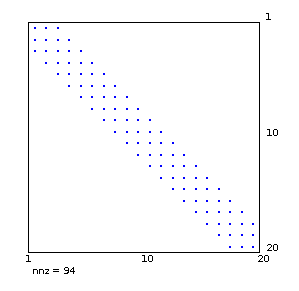
\includegraphics[scale=0.7]{figures/bound.png}
% \label{fig:bound}
% \end{figure}
% 
% Nous allons pr\'esenter trois exemples de fonction appartenant \`a la librairie; la fonction bien connue Rosenbrock, g\'en\'eralis\'ee \`a dimension variable, 
% une fonction trigonom\'etrique et une fonction utilisant les polynômes de Chebychev.
% 
% 
% 
% Comme les polynômes sont de plus en plus compliqu\'es \`a calculer quand la dimension augmente, le coût de $f$
% ne va pas être lin\'eaire par rapport \`a $n$.





\section{Pr\'ecision des objectifs}
Maintenant que nous avons pr\'esent\'e les algorithmes, nous pouvons mieux pr\'eciser les objectifs du pr\'esent travail.
Le but est d'adapter une libraire sous scilab et d'être capable de fournir les d\'eriv\'ees des fonctions qui v\'erifient
les complexit\'es expos\'ees en \ref{chap1:ordre}.
La difficult\'e des m\'ethodes r\'eside dans l'ensemble des op\'erations critiques : 
\begin{itemize}
\item $\nabla f(x)$
\item $\nabla f(x)\cdot u$
\item $\nabla^2 f(x)$
\item $\nabla^2 f(x)\cdot u$
\item $\nabla^3 f(x)\cdot u$
\item $\nabla^3 f(x)\cdot u\cdot v$
\item $\nabla^4 f(x)\cdot u\cdot v \cdot w$
\item d\'ecomposition de Cholesky $LDL^T = P(A+E)P^T$
\item r\'esolution du syst\`eme $LDL^Tx =b$
\end{itemize}

Nous voulons exploiter au mieux l'utilisation de DA afin d'obtenir des temps de calcul raisonnable pour les d\'eriv\'ees. 
De plus, il faut aussi pouvoir obtenir la d\'ecomposition de Cholesky modifi\'ee et être capable de r\'esoudre des syst\`emes triangulaires de mani\`ere
efficace sinon le gain ne servira \`a rien.
 Nous allons analyser les processus de la diff\'erentiation automatique dans 
l'obtention des d\'eriv\'ees. Nous verrons ainsi qu'il existe deux modes bien distincts pour les calculs et diff\'erentes techniques 
d'impl\'ementation. Puis, nous d\'etaillerons les choix au niveau des outils et des librairies pour les op\'erations critiques et leurs tests.
 Enfin, nous observerons les r\'esultats obtenus pour les temps d'ex\'ecution et l'efficacit\'e des m\'ethodes.


%Nous verrons aussi les limitations d'un outil (Tapenade).
% \subsection{Halley}
% Complexit\'e : $C(d_N)+$ Tenseur$\times$Vecteur






